\chapter{Quantum computing}
\label{chap:qc}
The field of quantum computing is split in two main branches: the development of quantum hardware and the study of algorithms that use such hardware.
Only the second branch is relevant for this thesis, and even so only a brief explanation is offered here.
This chapter is primarily based on the Qiskit textbook \cite{qiskit_textbook} and \citetitle{textbook_2nd} by \textcite{textbook_2nd}.
The discussion of variational quantum algorithms in section \ref{sec:vqa} is based on the review by \textcite{cerezo2021}.

\section{Quantum states}
\subsection{The qubit}
The quantum bit, the qubit, is the building block of quantum computing.
Like the classical binary digit, it can be either 0 or 1.
But being quantum, these are quantum states, $\ket{0}$ and $\ket{1}$\footnotemark{}, and the qubit can be in any superposition of these states.
The state of the qubit lies in a two-dimensional Hilbert space, and the states $\ket{0}$ and $\ket{1}$ are basis vectors, known as the computational basis states.
Thus, the state of a qubit can be expressed as
\begin{equation}
    \ket{\psi} = \alpha \ket{0} + \beta \ket{1} = \begin{pmatrix} \alpha \\ \beta \end{pmatrix},
    \label{eq:qubit}
\end{equation}
where $\alpha$ and $\beta$ are any numbers, even complex.
The only requirement is that the state is normalised, $\vert\alpha\vert^2 + \vert\beta\vert^2 = 1$.

\footnotetext{
    The $\ket{\cdot}$ notation is known as a ket and is used in quantum mechanics to denote a quantum state.
    It is effectively a column vector in a Hilbert space, whose inner product may be taken with a bra, $\bra{\cdot}$, to give a scalar.
    These inner products are then denoted by $\bra{\cdot}\ket{\cdot}$.
    Similarly, outer products are well-defined and denoted by $\ketbra{\cdot}{\cdot}$.
}

Normalisation is required due to the Born rule, as the absolute square of the coefficients is the probability of measuring the qubit in the corresponding basis state.
It is one of nature's great mysteries what exactly a measurement is, but in the quantum computational setting, it can be thought of as taking a random sample with the probabilities given by the coefficients, which can be done systematically.

\subsection{The Bloch sphere}
A useful tool for visualising the state of a qubit is the Bloch sphere.
First, it should be noted that states on the form \cref{eq:qubit} are not unique, only the relative complex phase matters.
There is a global phase which is not measurable, and thus not relevant to the state of the qubit.
Therefore, taking also the normalisation requirement into account, the state of the qubit can be expressed as
\begin{equation}
    \ket{\psi} = \cos\left(\frac{\theta}{2}\right) \ket{0} + e^{i\phi} \sin\left(\frac{\theta}{2}\right) \ket{1}
    \label{eq:bloch}
\end{equation}
where $\theta, \phi \in \mathbb{R}$.
Interpreting $\theta$ as the polar angle and $\phi$ the azimuthal angle, the state of the qubit can be identified with a point a sphere, known as the Bloch sphere.
There, the state $\ket{0}$ is typically thought of as the north pole, and $\ket{1}$ as the south pole.
\Cref{fig:bloch} shows the Bloch sphere with the state of the qubit in \cref{eq:bloch}.

\begin{figure}
    \centering
    \def\svgwidth{0.5\textwidth}
    \subimport{bloch}{bloch_sphere}
    \caption{
        The Bloch sphere.
        On it, the state of a single qubit state is represented by a point.
        The state $\ket{0}$ is the north pole, and $\ket{1}$ is the south pole.
        The latitudinal angle $\theta$ determines the probability of measuring the qubit in the state $\ket{0}$, while the longitudinal angle $\phi$ corresponds to the complex phase between the two basis states.
        From \cite{wikipedia_bloch}.
    }
    \label{fig:bloch}
\end{figure}

\subsection{Mixed states and density operators}
It is not only the superpositions of states that are important in quantum computing, but also the mixed states in which classical uncertainties manifest.
For the description of mixed states, the formalism of density operators is more useful than the state vector formalism.
In a mixed state, some classical probabilities $p_i$ are associated with the different states $\ket{\psi_i}$, and the state of the system is described by the density operator
\begin{equation}
    \rho = \sum_{i=1}^n p_i \ketbra{\psi_i}{\psi_i}
    \label{eq:density}
\end{equation}
where $\ket{\psi_i}$ are the states of the system, and $\bra{\psi_i}$ are the corresponding dual vectors.
Naturally, the $p_i$ must be non-negative and sum to one.
Furthermore, the density operator is positive semidefinite.
If there is no classical uncertainties, the state is called pure, and the density operator can be expressed a single ket-bra, $\rho = \ketbra{\psi}{\psi}$.

For a density operator, the diagonal elements are the probabilities of measuring the system in the corresponding basis states, and hence they are positive and the trace one.
Ergo, for a single qubit, the density operator can be expressed as
\begin{equation}
    \rho = \frac{1}{2} \left(I + x \sigma_x + y \sigma_y + z \sigma_z\right).
\end{equation}
Here, $x, y, z \in \mathbb{R}$, and $\sigma_x, \sigma_y, \sigma_z$ are the Pauli matrices,
\begin{equation}
    \sigma_x = \begin{pmatrix} 0 & 1 \\ 1 & 0 \end{pmatrix}, \quad
    \sigma_y = \begin{pmatrix} 0 & -i \\ i & 0 \end{pmatrix}, \quad
    \sigma_z = \begin{pmatrix} 1 & 0 \\ 0 & -1 \end{pmatrix},
    \label{eq:pauli}
\end{equation}
which together with the identity matrix serve as a basis for Hermitian $2\times 2$ matrices.
Being positive semidefinite, the determinant should be non-negative, and thus it can be showed that $x^2 + y^2 + z^2 \leq 1$.
This allows density operators to be interpreted as points on the Bloch sphere or indeed within it.
Notably, pure states lie on the surface, while mixed states lie within the sphere (or rather, the Bloch ball).
A pure quantum superposition of $\ket{0}$ and $\ket{1}$ with equal probabilities would have a complex phase and lie somewhere on the equator, while a statistical mixture with equal classical probabilities of being $\ket{0}$ and $\ket{1}$ would lie in its centre.

\subsection{Systems of multiple qubits}
Although the continuous nature of the qubit is indeed useful, the true power of quantum computers lie in how multiple qubits interact.
Having multiple qubits allows for the creation of entanglement, which is a key feature of quantum computing.

With just two qubits, there are four possible states, $\ket{00}, \ket{01}, \ket{10}, \ket{11}$.
Each of these four have their own probability amplitude, and thus their own probability of being measured.
A two-qubit system will therefore operate with four complex numbers.

Generally, the state of multiple qubits can be expressed using the tensor product as
\begin{equation}
    \ket{\psi_1 \psi_2 \cdots  \psi_n}
    = \ket{\psi_1} \ket{\psi_2} \cdots \ket{\psi_n}
    = \ket{\psi_1} \otimes \ket{\psi_2} \otimes \cdots \otimes \ket{\psi_n}
    \label{eq:tensor}.
\end{equation}
What makes this so powerful is that the state of a multi-qubit system can be anything on the form
\begin{equation}
    \ket{\psi_1 \psi_2 \cdots  \psi_n}
    = c_1 \ket{0\dots 00} + c_2 \ket{0\dots 01} + \cdots + c_{2^n} \ket{1\dots 11}
    = \begin{pmatrix}
        c_1 \\ c_2 \\ \vdots \\ c_{2^n}
    \end{pmatrix}
    \in \mathbb{C}^{2^n},
    \label{eq:superposition}
\end{equation}
which means that with $n$ qubits, the system can be in any superposition of the $2^n$ basis states.
Operating on several qubits then, one can do linear algebra in an exponentially large space.
This is the origin of the exponential speed-up of quantum computers.
\section{Quantum operations}
\label{sec:quantum_operations}
\subsection{Single-qubit gates}
To operate on one or more qubits, a unitary operation is applied to the state, where the unitarity is needed for states to remain normalised.
As they are unitary, any purity is preserved.
With the finite number of qubits, these operations can be expressed as matrices.
These operations are often thought of as gates, paralleling the classical gates in digital logic.
Mathematically, a unitary gate $U$ can be expressed as matrices acting on the state vector, $\ket{\psi}$, as
\begin{equation}
    \ket{\psi'} = U\ket{\psi},
\end{equation}
where $\ket{\psi'}$ is the resulting state.

The most basic gates are the Pauli gates, which are applications of the Pauli matrices from \cref{eq:pauli} and are as gates simply denoted as $X$, $Y$, and $Z$ respectively.
These gates can be seen as half turns around the $x$-, $y$- and $z$-axes, respectively, of the Bloch sphere.
The $X$-gate is also known as the NOT gate, as it mirrors the classical NOT gate by mapping $\ket{0}$ to $\ket{1}$ and vice versa.
It is however more general, being also applicable to superposition states.

The Hadamard gate,
\begin{equation}
    H = \frac{1}{\sqrt{2}} \begin{pmatrix} 1 & 1 \\ 1 & -1 \end{pmatrix},
\end{equation}
is a rotation around the line between the $x$- and $z$-axes by $\pi/2$.
It is an important gate in quantum computing, as it is used to create superpositions of the computational basis states.
Applied on the initial $\ket{0}$ state, it creates the entangled state $\frac{1}{\sqrt{2}}(\ket{0} + \ket{1})$.
Two consecutive applications thereof is a no-op, the second returns the state to the initial state, as can be seen from the matrix squaring to the identity.

The $R_X$-, $R_Y$- and $R_Z$-gates are rotations around the $x$-, $y$- and $z$-axes, respectively, by an arbitrary angle $\theta$:
\begin{align*}
    R_X(\theta) & = \begin{pmatrix} \cos\left(\frac{\theta}{2}\right) & -i \sin\left(\frac{\theta}{2}\right) \\ -i \sin\left(\frac{\theta}{2}\right) & \cos\left(\frac{\theta}{2}\right) \end{pmatrix}, \\
    R_Y(\theta) & = \begin{pmatrix} \cos\left(\frac{\theta}{2}\right) & -\sin\left(\frac{\theta}{2}\right) \\ \sin\left(\frac{\theta}{2}\right) & \cos\left(\frac{\theta}{2}\right) \end{pmatrix},      \\
    R_Z(\theta) & = \begin{pmatrix} e^{-i\frac{\theta}{2}} & 0 \\ 0 & e^{i\frac{\theta}{2}} \end{pmatrix}.
\end{align*}
These parametrised gates will be useful in \cref{sec:vqa}.

\subsection{Multi-qubit gates}
The most used multi-qubit gate is the controlled $X$-gate, also known as the CNOT.
Being controlled means that it only acts on the second qubit if the first qubit is in the state $\ket{1}$.
Of course, the first qubit may be in a superposition, and the CNOT this way allows for the creation of entanglement between the two qubits.
If the first qubit has probability amplitude $\alpha$ of being in the state $\ket{1}$, the second qubit will have probability amplitude $\alpha$ of being flipped.
The CNOT gate can be expressed in matrix form as
\begin{equation}
    \text{CNOT} = \begin{pmatrix} 1 & 0 & 0 & 0 \\ 0 & 1 & 0 & 0 \\ 0 & 0 & 0 & 1 \\ 0 & 0 & 1 & 0 \end{pmatrix}.
\end{equation}

In theory, any unitary single-qubit operation can be controlled.
Another interesting two-qubit gate is the controlled $Z$-gate, CZ, expressible as the matrix
\begin{equation}
    \text{CZ} = \begin{pmatrix} 1 & 0 & 0 & 0 \\ 0 & 1 & 0 & 0 \\ 0 & 0 & 1 & 0 \\ 0 & 0 & 0 & -1 \end{pmatrix}.
\end{equation}
Because it only alters the amplitude of $\ket{11}$, it does not actually matter which qubit is the control and which is the target.



\subsection{Observables and measurements}
For an output to be obtained from a quantum computer, a measurement must be performed.
This is typically done at the end of all operations and of all qubits, thus yielding a single output of zeros and ones, a bit-string.
It is important to note that the measurement is not a deterministic process, but rather a probabilistic one.
Often, the underlying probabilities are what is of interest.
Therefore, many measurements are performed.
Usually, these results are averaged to obtain an estimate, but more complicated post-processing methods are also possible.
For instance, neural networks have shown useful properties in regard of reducing variance in the estimates, though at the cost of some bias \cite{torlai2020}.

The $Z$-basis is the canonical basis for measurements, but any other basis can be used, at least in theory.
Often, only canonical basis measurements are implemented in the hardware.
Using another basis can be done by properly modifying the state before the measurement; a change of basis can simply be implemented by a unitary operation.

Measurements may be done in the middle of operations and be used to control the operations.
If the qubits are entangled, measuring one will affect the measurement probabilities of others.
Using such intermediate measurements is a way of introducing non-linearities in the otherwise unitary nature of the quantum world.


\subsection{Quantum circuits}
The operations on qubits are often described using quantum circuits, which are a graphical representation of the operations on the qubits, the quantum algorithms.
They are read from left to right.
It is standard procedure to assume all qubits start in the state $\ket{0}$.
Gates are generally written as boxes with the name of the gate inside.

A simple example is the circuit
\begin{equation}
    \begin{quantikz}
        \lstick{$\ket{0}$} & \gate{H} & \qw \\
        \lstick{$\ket{0}$} & \gate{H} & \qw
    \end{quantikz},
\end{equation}
which prepares the state $\frac{1}{2}(\ket{00} + \ket{01} + \ket{10} + \ket{11})$.
This is a pure state with no entanglement, and so the measurement probabilities of the two qubits are independent.

Slightly more interesting is the circuit
\begin{equation}
    \begin{quantikz}
        \lstick{$\ket{0}$} & \gate{H} & \ctrl{1} & \qw \\
        \lstick{$\ket{0}$} & \qw & \targ{} & \qw
    \end{quantikz}
\end{equation}
in which the first qubit is put into a superposition using the Hadamard gate before a CNOT gate is applied to the second, controlled on the first.
This creates the state $\frac{1}{\sqrt{2}}\left(\ket{00} + \ket{11}\right)$.
The measurement probabilities of the two qubits are now correlated; if the first qubit is measured to be $\ket{1}$, the second will always be $\ket{1}$ and vice versa.
The probability of measuring the qubits to be different is nil.

To create a mixed state, an intermediate measurement can be used to control a gate.
For instance, the circuit
\begin{equation}
    \begin{quantikz}
        \lstick{$\ket{0}$} & \gate{H} & \meter{} & \cwbend{1} \\
        \lstick{$\ket{0}$} & \qw & \qw & \gate{X} & \qw
    \end{quantikz}
\end{equation}
places the second qubit in the mixed state $\frac{1}{2}(\ketbra{0}{0} + \ketbra{1}{1})$.
If it were immediately to be measured, it would have a 50\% chance of being $\ket{0}$ and a 50\% chance of being $\ket{1}$.
The uncertainty is only classical, and it could therefore not be used to create entanglement or for any other quantum spookiness.

\subsection{Quantum supremacy}
\begin{sloppypar}
    Exponential speed-ups do not come for free.
    Quantum computers do only solve certain problems more efficiently than classical computers, and finding the algorithms to do so is no easy task.
    \sloppy Shor's algorithm has time complexity $O((\log N)^2 (\log \log N) (\log \log \log N))$ while the most efficient known classical algorithm has time complexity $O(\exp{1.9(\log N)^{1/3} \text{} (\log \log N)^{2/3}})$.
    To solve linear system algorithms, the HHL algorithm has time complexity $O(\log(N)\kappa^2)$ where $\kappa$ is the condition number, which is an exponential speed-up over the fastest known classical algorithm has time complexity $O(N \kappa)$.
    Still, discovering these algorithms is not trivial.
\end{sloppypar}

Polynomial speed-ups are also found.
For example, the Grover algorithm which is used to search for an element in an unsorted list has time complexity $O(\sqrt{N})$.
Classically, this can not be done in less than $O(N)$ time.
This algorithm, or the more general amplitude amplification on which it builds, solves a very general problem and is often used a subroutine to achieve quadratic speed-ups in other algorithms.
Being only a quadratic speed-up, it is not as impressive as the exponential speed-ups,
and achieving quantum supremacy in that manner would require larger quantum computers than if the speed-up were exponential.

It is proven that the class of problems quantum computers can solve in polynomial time (with high probability), BQP, contains the complexity class P.
This follows from the fact than quantum computers can do any classical algorithm.
Since quantum computers can solve problems like integer factorisation and discrete logarithms efficiently, it is believed that BQP is strictly greater than P, but as whether P=NP remains unknown, these problems could actually be in P.
In a similar vein, NP-complete problems are believed to lie outside BQP.
\section{Limitations of NISQ hardware}
\label{sec:nisq}
Quantum hardware have been physically realised and even outperforms classical computers in very contrived situations \cite{arute2019, zhong2020, madsen2022}, but the hardware is still very limited.
The hardware is limited in the number of qubits, the connectivity between the qubits, and the noise and decoherence of the qubits.
It is believed that quantum hardware will continue to improve and eventually perform demanding algorithms like Shor's for large numbers.
Once enough qubits are available and error rates low enough, error correction schemes can be implemented, permitting fault-tolerant quantum computing and truly enable quantum supremacy.
Still, the era dubbed NISQ (Noisy Intermediate-Scale Quantum) is the first step, and to make use of the hardware, the inherent noise and its consequences must be understood, and algorithms must take the following limitations into consideration.

\subsection{Quantum channels and decoherent noise}
The unitary gates from \cref{sec:quantum_operations} are an idealisation, and in reality, the gates are not perfect.
A more realistic description of the gates is given by quantum channels, which can take noise into account.
In an unmeasured, ideal quantum system, the state evolution is veritably unitary, but as the system in practice does interact with the environment, this can be modelled as a quantum channel in which traditionally probabilistic noise is introduced.

Take the $X$-gate as an example.
If the fails to apply with probability $p$, the resulting density operator $\rho'$ can be expressed as
\begin{equation}
    \rho' = p\rho + (1-p)X\rho X^\dagger,
\end{equation}
where $\rho$ is the initial density.
Such a channel has eigenvalues $p$ and $1-2p$, where $I$ and $X$ share the former and $Y$and $Z$ the latter.
Consequently, states with $Y$- or $Z$-components will have mixing introduced.
Geometrically, this can be interpreted as contraction of states on the Bloch sphere towards the centre, illustrated in \cref{fig:noise_bloch}.

\begin{figure}
    \centering
    \begin{tikzpicture}
        \begin{groupplot}[
                group style={
                        group size=2 by 1,
                        horizontal sep=0pt,
                    },
                width=\textwidth,
                % height=30 cm,
                ymin = -1.5, ymax = 1.5,
                xmin = -1.5, xmax = 1.5,
                zmin = -1.5, zmax = 1.5,
                % grid=major,
                axis equal,
                axis lines = center,
                xlabel = {$x$},
                ylabel = {$y$},
                zlabel = {$z$},
                xtick = {-1, 0, 1},
                ytick = {-1, 0, 1},
                ztick = {-1, 0, 1},
                % enlargelimits=0.3,
                view/h=120,
                view/v=30,
                scale uniformly strategy=units only,
            ]
            \nextgroupplot
            \addplot3[
                opacity = 0.35,
                surf,
                fill=white, point meta=0,
                z buffer = sort,
                samples = 21,
                variable = \u,
                variable y = \v,
                domain = 0:180,
                y domain = 0:360,
            ]
            ({cos(u)*sin(v)}, {sin(u)*sin(v)}, {cos(v)});;
            \nextgroupplot[xshift=-3cm]
            \addplot3[
                opacity = 0.35,
                surf,
                fill=white, point meta=0,
                z buffer = sort,
                samples = 21,
                variable = \u,
                variable y = \v,
                domain = 0:180,
                y domain = 0:360,
            ]
            ({cos(u)*sin(v)}, {0.6*sin(u)*sin(v)}, {0.6*cos(v)});
        \end{groupplot}
        % add arrow from north on fig 1 to north on fig 2 
        \draw[->, shorten >=0.5cm,shorten <=1cm]
        ([yshift=-2.5cm] group c1r1.north)
        edge[bend left]
        node[midway,above] {\footnotesize Noisy $X$-gate}
        ([yshift=-2.5cm] group c2r1.north);
    \end{tikzpicture}
    \caption{
        Illustration of applying a noisy $X$-gate on the Bloch sphere.
        The left plot shows the set of all pure states, the Bloch sphere.
        On the right, the same set of states is shown after the application of a noisy $X$-gate with probability $p=0.2$ of failing.
        There, the $y$- and $z$-axes are contracted towards the centre by a factor $1-2p=0.6$, introducing mixing.
    }
    \label{fig:noise_bloch}
\end{figure}

Any physical gate will suffer some such noise, and so the tendency will be for states to degenerate towards the mixed centre of the Bloch sphere (or its higher-dimensional analogue).
Furthermore, measurements, letting a qubit idle when operating on others and even the preparation of the initial state $\ket{0}^{\otimes n}$ will suffer from decoherence.

This noise is very hard to avoid, as controlling the qubits necessarily requires some interaction with the environment.
Additionally, to operate on multiple qubits, a connection between them is required, which too will suffer from noise.
Nature tends to work against large quantum systems, made evident by the absence of quantum effects in regular life.

Due to the multiplicative effect of noise, the overall degeneracy will increase exponentially with the number of operations.
This means that there will be limits to the number of operations that can be performed before the system becomes unusable, assuming no error-correction is done.

\subsection{Coherent noise}
There may also be systematic errors in the unitary gates applied.
This kind of noise, known as coherent noise does not need quantum channels to be modelled, but may rather be modelled simply by slightly different unitary gates.
Here too, the $X$-gate can serve as an example.
Such a gate is typically implemented by applying a Hamiltonian for some time, requiring calibration of said time.
%
If it is not calibrated correctly, the effective operation will be a rotation that slightly deviates from the intended half turn.
When a gate like the $X$-gate is applied many times, even small errors will add up, which could cause an overall rotation of the state by a significant angle.

\begin{figure}
    \centering
    \begin{tikzpicture}
        \begin{axis}[
                width=0.6\textwidth,
                height=0.4\textwidth,
                xlabel = {Number of $X$-gates applied},
                ylabel = {Correct measurements (\%)},
                y filter/.code={\pgfmathparse{#1*100}\pgfmathresult},
                grid = major,
                % ytick = {0.1, 0.2, 0.3, 0.4, 0.5, 0.6, 0.7, 0.8, 0.9, 1},
            ]
            \addplot[
                color = blue,
                mark = none,
                % samples = 100,
                % domain = 0:100,
            ]
            table[x = n, y = p, col sep=comma] {../code/noise_fig/noise.csv};
            % add exponential dampening to the plot
            \addplot[
                color = gray,
                dashed,
                mark = none,
                samples = 100,
                domain = 0:1000,
            ]
            {0.5*(1+(1-2*0.003)^x)};
            \addplot[
                color = gray,
                dashed,
                mark = none,
                samples = 100,
                domain = 0:1000,
            ]
            {0.5*(1-(1-2*0.003)^x)};
            \addplot[
                color = gray,
                densely dotted,
                mark = none,
                samples = 100,
                domain = 0:1000,
            ]
            {0.5*(1 + cos(x))};
            \addplot[
                color = black,
                solid,
                mark = none,
                samples = 100,
                domain = 0:1000,
            ]
            {0.5*(1+cos(x)*(1-2*0.003)^x)};
        \end{axis}
    \end{tikzpicture}
    \caption{
        Proportion of correct measurements of a qubit after applying several noisy $X$-gates.
        The error in the rotation is \ang{1}, while the probability of failing to apply the gate is $p=0.3\%$.
        For each number of gates, the measurement is repeated 1000 times.
        The coherent error causes a sinusoidal behaviour, in which 180 rotations causes the overall rotation to be completely opposite.
        The decoherent error causes an exponential dampening, as the state becomes more and more mixed.
        The wiggly pattern stems from the shot noise, simply classical randomness stemming from the probabilistic measurement with a finite number of samples.
    }
    \label{fig:noise_graph}
\end{figure}

\Cref{fig:noise_graph} shows the effects of both coherent and decoherent noise on the measurement of a qubit after applying several noisy $X$-gates.
Clearly, information is quickly lost as the quantum state ends up different from what is expected and as the system becomes more and more mixed, losing quantum properties and instead obeying classical probabilities.
Even though current hardware suffers much less noise than the figure shows, NISQ algorithms must nonetheless be shallow, meaning that the amount of gates applied before measurement is small.
There are more sources of noise than the two included in the figure, and having to deal with multiple qubits certainly does not help.

\subsection{Qubit counts and connectivity}
\begin{figure}[b]
    \centering
    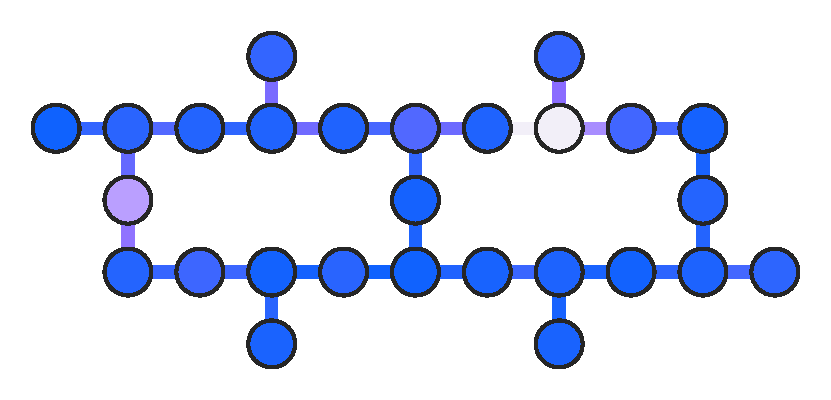
\includegraphics[width=0.65\textwidth]{connectivity.pdf}
    \caption{
        Qubit connectivity and error rates in IBM's 127-qubit Eagle r3 chip \cite{ibm_eagle}.
        Brighter coloured nodes indicate more $X$-errors, while brighter edges indicate more CNOT-errors.
        Only the CNOT-, $R_Z$-, $X$- and $\sqrt{X}$-gates are available.
    }
    \label{fig:connectivity}
\end{figure}
Another limiting factor is the amount of qubits.
Current hardware has around 10 to 100, which though still may be enough to express states too large for classical computers, is not enough to perform the most demanding algorithms.
Recent estimates find that millions of noisy qubits would be needed to break RSA encryption \cite{gidney2021}.

Another current limitation is the connectivity between the qubits.
Consider for example the connectivity graph in \cref{fig:connectivity}.
Qubits are generally only linked to two neighbouring qubits.
Moreover, only a basis set of gates will be directly available.
All this means that qubits may have to be swapped, often many times, and that multiple gates may be needed where only was intended.
This increases circuit depths, which in turn exacerbates the effects of noise.

\section{Variational quantum algorithms}
\label{sec:vqa}
Variational quantum algorithms (VQAs) are envisioned as the most likely candidate for quantum advantage to be achieved in the NISQ-era.
By optimising a set of parameters that describe the quantum circuit, classical optimisation techniques are applicable, and only using the quantum hardware for what can be interpreted as function calls limits the circuit depths needed.
Running the same circuit many times with different parameters and inputs in a classical-quantum-hybrid fashion, rather than a complete quantum implementation, means that the quantum operations can be simple enough for the noise and decoherence to be manageable.
This loop of running the circuit, measuring the output to evaluate a cost, optimising and updating the parameters is pictured in \cref{fig:vqa}.

\begin{figure}
\centering
\begin{tikzpicture}
\tikzstyle{box} = [
rectangle,
draw,
dashed,
rounded corners,
outer sep=0.2cm,
inner sep=0.2cm,
fill = white,
]
\tikzset{%
    cascaded/.style = {%
            general shadow = {%
                    shadow scale = 1,
                    shadow xshift = -1.5ex,
                    shadow yshift = - 1.5ex,
                    draw,
                    % thick,
                    fill = white,
                    draw opacity = 0.1,
                },
            general shadow = {%
                    shadow scale = 1,
                    shadow xshift = -1ex,
                    shadow yshift = - 1ex,
                    draw,
                    % thick,
                    fill = white,
                    draw opacity = 0.2,
                },
            general shadow = {%
                    shadow scale = 1,
                    shadow xshift = -.5ex,
                    shadow yshift = -.5ex,
                    draw,
                    % thick,
                    fill = white,
                    draw opacity = 0.4
                },
            % fill = white,
            % draw,
            % thick,
            % minimum width = 1.5cm,
            % minimum height = 2cm
        }
}

\node[box, cascaded, label=below:{Parametrised circuit}] (qc) at (-4, -1) {
        \begin{quantikz}[
                % manually have to avoid inheriting the node style
                solid,
                rounded corners=0,
                outer sep=0,
                inner sep=0.2cm,
            ]
            \lstick{$\ket{0}$}
            &
            \gate[wires=3, nwires=2]{U(\bm{\theta})}
            &
            \meter{}
            \rstick[wires=3]{\rotatebox{90}{Measurements}}
            \\
            \lstick{\vdots} & &
            \\
            \lstick{$\ket{0}$} & \qw & \meter{}
        \end{quantikz}
    };
\node[box, label=below:{Cost and its gradient}] (cf) at (2, -1) {
        $
            \begin{+matrix}
            C(\bm{\theta}), \\
            \nabla_{\bm{\theta}} C(\bm{\theta})
            \end{+matrix}
        $
    };
\node[box] (opt) at (2, 2) {Classical optimiser};
\node[box] (up) at (-4, 2) {Updated $\bm{\theta}$};
\draw[->] (qc) -- (cf);
\draw[->] (cf) -- (opt);
\draw[->] (opt) -- (up);
\draw[->] (up) -- (qc);
\end{tikzpicture}
\caption{
    The general structure of a VQA.
    Given some initial parameters $\bm{\theta}$, a parametrised quantum circuit is run multiple times on quantum hardware, after which a cost $C(\bm{\theta})$ function is calculated based on the measurements.
    The parameters of the quantum circuit are subsequently updated by a classical optimiser, and the process is repeated until some convergence criterion is met.
}
\label{fig:vqa}
\end{figure}

Generally, VQAs start with defining a cost function, depending on some input data (states) and the parametrised circuit, to be minimised with respect to the parameters of the quantum circuit.
For example, the cost function for the variational quantum eigensolver (VQE) is the expectation value of some Hamiltonian, which is the energy of a quantum-mechanical system, such as different molecules....
The cost function should be meaningful in the sense that the minimum coincides with the optimal solution to the problem, and that lower values generally imply better solutions.
Additionally, the cost function should be complicated enough to warrant quantum computation by not being easily calculated on classical hardware, while still having few enough parameters to be efficiently optimised.

Important to the success of a VQA is the choice of the quantum circuit.
The circuit selected is known as the ansatz, and there are a plethora of different ansätze to choose from.
An example are hardware-efficient ansätze, which, as the name implies, is a general term used for ansätze designed in accordance with the hardware properties of a given quantum computer, taking for instance the physical gates available into account and minimising the circuit depth.
Other ansätze may be problem-specific, like the quantum alternating operator ansatz used for the quantum approximate optimisation algorithm (QAOA) (both sharing the QAOA acronym, confusingly), while others are more general and can be used to solve a variety of problems.

The optimisation of the cost function is often done with gradient descent methods.
To evaluate the gradient of the quantum circuit with respect to the parameters, the very convenient parameter shift rule is commonly used.
Though appearing almost as a finite difference scheme, relying on evaluating the circuit with slightly shifted parameters, it is indeed an exact formula.
Not having to rely on finite differences is a major advantage, as the effects of small changes in parameters would quickly be drowned out in noise.
Furthermore, it may be used recursively to evaluate higher order derivatives, which allows the usage of more advanced optimisation methods like the Newton method that requires the Hessian.

Applications of VQAs are numerous.
A typical example is finding the ground state of a Hamiltonian for a molecule.
Such problems are exponential in the particle count, and thus intractable on classical hardware for larger molecules, while the problem of evaluating the Hamiltonian on quantum hardware is typically polynomial.
VQAs are also well suited for general mathematical problems and optimisation, with another common example being QAOA for the max-cut problem.

Still, there are many difficulties when applying VQAs.
Exponentially vanishing gradients, known as barren plateaus, are a common occurrence, making optimisation futile.
The choosing of the ansatz determines the performance and feasibility of the algorithms, and there are many strategies and options.
Some rely on exploiting the specific quantum hardware's properties, while others use the specifics of the problem at hand.
Finally, the inherent noise and errors on near-term hardware will still be a problem and limit circuit depths.




